\documentclass[10pt]{beamer}
\usetheme{metropolis}           % Use metropolis theme
\usepackage[utf8]{inputenc}
\usepackage{amsmath,amsfonts,amssymb}
\usepackage{dsfont}
\usepackage{graphicx}
\usepackage{caption}
\usefonttheme[onlymath]{serif}


\title{Théorème de Hille-Yosida et applications}
\date{\today}
\author{Sacha Ben-Arous, Clément Robiez, Quentin Verrier}
\institute{ENS Paris-Saclay}
\begin{document}
  \maketitle
\begin{frame}
\tableofcontents
\end{frame}  


\section{Théorème de Hille-Yosida}
\begin{frame}{Définitions}
On travaille dans un espace de Hilbert $H$. On considère un opérateur linéaire non borné (i.e non continu) $A : D(A)\rightarrow H$.
\begin{itemize}
\item[•]  $A$ est monotone si $\forall v \in D(A), \ \left<Av,v\right> \geq 0$ \\ ~ \\
\item[•] $A$ est maximal si $\forall f\in H, \ \exists u\in D(A), \ u + Au=f$ 
\end{itemize}
\end{frame}


\begin{frame}{Propriétés fondamentales}
Si $A$ est un opérateur maximal monotone, alors :
\begin{itemize}
\item[•]  $D(A)$ est dense dans $H$ 
\item[•] Le graphe de $A$ est fermé 
\item[•] $\forall \lambda > 0, \ (I+\lambda A)$ est une bijection, et $\|(I+\lambda A)^{-1}\|_{\mathcal{L}(H)} \leq 1 $
\end{itemize}
\end{frame}


\begin{frame}{Outils de la preuve}
Soit $A$ est un opérateur maximal monotone, on note pour $\lambda > 0$ :
\begin{itemize}
\item<1->[•] $J_{\lambda} := (I+\lambda A)^{-1}$ la résolvante de $A$
\item<1->[•] $A_{\lambda} := \frac{1}{\lambda}(I-J_{\lambda})$ l'approximation de Yosida de $A$ 
\end{itemize}
\underline{Rq} : $A_{\lambda}$ est continue et définie sur $H$. \\ ~ \\
\onslide<2->{
On a les propriétés suivantes : 
\begin{itemize}
\item[•] $A_\lambda v = A(J_\lambda v) $ et $ A_\lambda v = J_\lambda (A v) $
\item[•] $\lim\limits_{\lambda\to 0} J_\lambda v = v$ et $\lim\limits_{\lambda\to 0} A_\lambda v = Av$
\item[•] $\|A_\lambda v \| \leq \frac{1}{\lambda}\| v \|$ et $\|A_\lambda v \| \leq \| A v \|$
\end{itemize}
}
\end{frame}


\begin{frame}{Théorème de Hille-Yosida}
\textbf{Théorème (Hille-Yosida) : \\}
Soit $A$ un opérateur maximal monotone.\\
 Alors, $\forall u_0 \in D(A), \ \exists ! u \in \mathcal{C}^1([0,+\infty[,H) \cap\mathcal{C}([0,+\infty[,D(A)) $ tel que : \\ ~ \\
$(*) \begin{cases}\displaystyle \frac{du}{dt} +Au = 0 \text{\ \ \ \ sur } [0,+\infty[ \\ u(0)=u_0 \end{cases}$ \\ ~ \\ ~ \\
De plus  $\forall t \geq 0$, $\|u(t)\|\leq \|u_0\| \ $ et $\ \displaystyle \|\frac{du}{dt}\| \leq  \|Au_0\|$
\end{frame}


\begin{frame}{Preuve (1) : Unicité}
Soient $u_1,u_2$ solutions de $(*)$, on a : 
\begin{eqnarray*}  \frac{1}{2}\frac{d}{dt}|u_1-u_2|^2  &=& \left< \frac{d}{dt}(u_1-u_2),(u_1-u_2)\right> \\
&=&-\left< A(u_1-u_2),(u_1-u_2)\right> \ \leq \ 0
\end{eqnarray*}
\\ ~ \\
Or $u_1(0)=u_2(0)=u_0$, donc $ \forall t \geq 0, \ u_1(t)=u_2(t)$
\end{frame}


\begin{frame}{Preuve (2) : Approximations}
Soit $\lambda \geq 0$ : \\ ~ \\
$(**) \begin{cases}\displaystyle \frac{d}{dt}u_\lambda +A_\lambda u_\lambda = 0 \\ u_\lambda(0)=u_0 \end{cases}$ \\ ~ \\ 
Il existe $u_\lambda$ solution $\mathcal{C}^\infty$ de $(**)$ par C-L. \\ ~ \\ 
On a $\left< A_\lambda u_\lambda,u_\lambda\right> \geq 0$ et $\frac{1}{2}\frac{d}{dt}|u_\lambda|^2 \leq 0$ donc $|u_\lambda|\leq u_0$. \\ ~ \\
Par le même raisonnement, on obtient la décroissance de toutes les dérivées.
\end{frame}

\begin{frame}{Preuve (3) et (4) : Convergence}
Soit $\lambda, \mu \geq 0$, on a de même  $\frac{1}{2}\frac{d}{dt}|u_\lambda-u_\mu|^2 \leq 2(\lambda + \mu) |Au_0|^2$, et en intégrant on obtient : \\~ \\
$|u_\lambda -u_\mu| \leq 2 \sqrt{(\lambda + \mu)t}\ |Au_0|$\\~ \\ 

Donc sur tout segment $[0,T]$ on a une suite de Cauchy, sur lequel la convergence va être uniforme vers $u \in \mathcal{C}([0,+\infty[,H)$. \\~\\ 

Si de plus $u_0 \in D(A^2)$, on peut refaire le même raisonnement avec les dérivées pour obtenir $u \in \mathcal{C}^1([0,+\infty[,H)$. \\~\\ 
\end{frame}


\begin{frame}{Preuve (5) : Densité}
On remarque que $\lim\limits_{\lambda\to 0} J_\lambda u_\lambda= u$, et de plus $\displaystyle \frac{du_\lambda}{dt} + A(J_\lambda u_\lambda)=0$. \\~ \\
Alors, $A$ étant fermé, on en déduit que $\forall t \geq 0, u(t) \in D(A)$, et $u \in \mathcal{C}([0,+\infty[,D(A))$, donc que $u$ est solution de $(*)$.\\~ \\
\onslide<2->{\textbf{Lemme :} \\
Soit $u_0 \in D(A)$, en notant $u_0' := J_\lambda u_0 \in D(A)$, on a $u_0' + \lambda A u_0' = u_0$. \\~\\
Alors $u_0' \in D(A^2)$, et $\lim\limits_{\lambda\to 0} J_\lambda u_0 = u_0$ et $\lim\limits_{\lambda\to 0} J_\lambda Au_0 = Au_0$ , ce qui donne la densité de $D(A^2)$ dans $D(A)$.}
\end{frame}

\begin{frame}{Preuve (6) : Densité}

Soit $(u_{0,n})_{n\in \mathbb{N}} \in D(A^2)^\mathbb{N}$ qui tend vers $u_0$ pour la norme du graphe. On considère les solutions $(u_{n})_{n\in \mathbb{N}}$ associées par l'étape $(5)$. Par décroissance, on a \\~\\
$\begin{cases} |u_{n}(t) - u_{m}(t)| \leq |u_{0,n}-u_{0,m}| \to 0 \\ \displaystyle |\frac{du_{n}}{dt}(t) - \frac{du_{m}}{dt}(t)|\leq |Au_{0,n}-Au_{0,m}| \to 0 \end{cases}$ \\ ~ \\ 

Alors convergence uniforme sur $\mathbb{R}^+$, leur limite vérifie $u\in \mathcal{C}^1([0,+\infty[,H)$ \\~\\
Comme $A$ est fermé, $\forall t \geq 0, u(t) \in D(A)$, et $u$ satisfait le problème initial, ce qui achève la preuve. \\~\\ \qed
\end{frame}
\section{Équation de la chaleur}

\begin{frame}{Présentation du problème}
$(*)\begin{cases} \displaystyle \Delta u = \frac{du}{dt} \\ u(0)=u_0(x) \ \ \text{où } \ u_0 \in \mathcal{L}^2(\Omega) \end{cases}$ \\ ~ \\ ~ \\ 

On veut appliquer Hille-Yosida avec $A=-\Delta$, sur l'espace de Hilbert $\mathcal{L}^2(\Omega)$, avec $D(A)= \mathcal{H}^2(\Omega)$, sur $\Omega$ qui est un ouvert régulier de $\mathbb{R}^n$.
\end{frame}



\begin{frame}{Cas $\Omega=\mathbb{R}^n$}
La transformée de Fourier est plus forte que Hille-Yosida dans le cas particulier où $\Omega=\mathbb{R}^n$, car on obtient une forme explicite de la solution. On raisonne par analyse synthèse : \\ ~ \\ ~ \\  
$\displaystyle \widehat{\frac{du}{dt}}-\widehat{\Delta u}=0$, or on a $\widehat{\frac{du}{dt}}=\frac{d\hat{u}}{dt}$ et $\widehat{\Delta u}=-|\xi|^2\hat{u}$ \\ ~ \\ ~ \\ 

On obtient alors $\widehat{u}=\widehat{u_0} \ e^{-|\xi|^2t}$, et donc $u=\text{TF}^{-1}(\widehat{u_0} \ e^{-|\xi|^2t})$
\end{frame}



\begin{frame}{Noyau de la chaleur}
Par les calculs, on obtient $u=\frac{1}{(2\pi)^d}  \displaystyle \int_{\mathbb{R}^d} u_0(y)\sqrt{\frac{\pi}{t}}^d e^{-\frac{|x-y|^2}{4t}} \, \mathrm{d}y $\\ ~ \\ 
On reconnait un produit de convolution entre $u_0$ et $\mathcal{H}_t$ le noyau de la chaleur. \\ ~ \\ 

$\mathcal{H}_t := \frac{1}{\sqrt{(4\pi t)^d}} e^{-\frac{|x|^2}{4t}}$ \\ ~ \\ 

Réciproquement, cette solution vérifie $(*)$.
\end{frame}


\begin{frame}{Cas général}
On veut résoudre dans $\mathcal{H}^2(\Omega)$. La monotonie du laplacien est immédiate, la partie difficile étant la maximalité : \\ ~ \\ 
$-\Delta u +u = f \ \text{où} \ f \in \mathcal{L}^2(\Omega) $   \\ ~ \\ 
Il est facile de prouver l'existence de solution dans $\mathcal{H}^1(\Omega)$ grâce au théorème de Lax-Milgram :\\ ~ \\ 
$\exists !\  u\in\mathcal{H}^1(\Omega), \ \forall v \in \mathcal{H}^1(\Omega), \displaystyle \int_{\Omega} \nabla u \cdot \nabla v \,  + \int_{\Omega} u v =  \int_{\Omega} f v  \, $
\end{frame}



\section{Régularité elliptique}

\begin{frame}{Théorème (Dirichlet)}
\textbf{Théorème (version Dirichlet) :} Soit $\Omega$ un ouvert de classe $\mathcal{C}^2$, de frontière $\Gamma$ bornée. Si $f \in \mathcal{L}^2(\Omega)$ et $u\in \mathcal{H}^1_0(\Omega)$ tq : \\ ~ \\  $\forall v \in \mathcal{H}^1_0(\Omega), \ \displaystyle \int_{\Omega} \nabla u \cdot \nabla v \,  + \int_{\Omega} u v =  \int_{\Omega} f v  \, \ \ \ (*) $\\ ~ \\ 
Alors $u\in \mathcal{H}^2(\Omega)$. \\~\\

\underline{Rq }: Ce théorème est encore valide si on ne suppose que $u,v\in\mathcal{H}^1(\Omega)$ et qu'on impose la valeur du gradient sur la frontière. Il s'agit des conditions de Neumann.
\end{frame}


\begin{frame}{Idée de la preuve}
On étudie la cas $\Omega=\mathbb{R}^n$ et  $\Omega=\mathbb{R}^n_+(=\mathbb{R}^{n-1}\times ]0;+\infty[)$, qui contiennent l'essentiel de la preuve dans le cas général. \\ ~ \\ 

On se servira de $\displaystyle D_hu(x):=\frac{u(x+h)-u(x)}{|h|}$ quand cet objet a un sens.

\end{frame}


\begin{frame}{Lemme}
\textbf{Lemme :}
$\forall v \in \mathcal{H}^1(\Omega), \ h \ \| \ \Gamma$, on a $\ \|D_hv\|_{\mathcal{L}^2(\Omega)} \leq \|\nabla v\|_{\mathcal{L}^2(\Omega)}  $ \\~\\

\textbf{Preuve :} On se rammène à $\mathcal{C}^1\cap \mathcal{H}^1(\Omega)$ par densité de cet ensemble. \\~\\
On a $D_hv(x) = \displaystyle \frac{1}{|h|}\int_0^1 \nabla v(x+th).h \,\mathrm{d}t $, et comme de plus : \\~\\

$\displaystyle \left | \int_0^1 \nabla v(x+th).h \,\mathrm{d}t \right |^2 \leq |h|^2 \int_0^1 |\nabla v(x+th)|^2 \,\mathrm{d}t $ par C-S, on obtient : \\~\\

$\|D_hv\|^2_{\mathcal{L}^2(\Omega)} \leq \displaystyle \int_{\Omega} \int_0^1 | \nabla v(x+th)|^2 \,\mathrm{d}t \,\mathrm{d}x \leq \| \nabla v\|^2_{\mathcal{L}^2(\Omega)}$ \\~\\

en utilisant un changement de variable et Fubini-Tonelli. On conclut dans le cas général par continuité de la norme.

\end{frame}


\begin{frame}{Cas $\Omega=\mathbb{R}^n$ ou $\mathbb{R}^n_+$ (1)}
On applique $(*)$ avec $v=D_{-h}D_hu$, ce qui donne  : \\~\\

$ \displaystyle \int_{\Omega} |\nabla D_h u|^2 \,  + \int_{\Omega} |D_hu|^2 =  \int_{\Omega} f D_{-h}D_hu  \,$ \\~\\

Par Cauchy-Schwarz on obtient : \\~\\ 

$\|D_hu\|^2_{\mathcal{H}^1} \leq \|f\|_2 \|D_{-h}(D_hu)\|_2 $, ce qui donne avec le lemme précédent : \\~\\

$\|D_hu\|_{\mathcal{H}^1} \leq \|f\|_2 $
\end{frame}


\begin{frame}{Cas $\Omega=\mathbb{R}^n$ ou $\mathbb{R}^n_+$ (2)}
On se donne alors $\varphi \in \mathcal{C}^\infty_c(\Omega)$, et on a : \\~\\

$\displaystyle \left |\int uD_{-h} (\frac{\partial \varphi}{\partial x_j})\, \right | = \displaystyle \left | - \int D_h (\frac{\partial u}{\partial x_j} )\varphi \, \right | \leq \|f\|_2 \|\varphi\|_2 $ \\~\\

En passant à la limite sur $h$, on obtient $\forall 1\leq j \leq n$ et $1 \leq k \leq n-1$ : \\~\\

$\left |\displaystyle \int u \frac{\partial^2 \varphi}{\partial x_j \partial x_k} \, \right | \leq \|f\|_2 \|\varphi\|_2 $ \\~\\

Sur $\mathbb{R}^n$, $k=n$ ne pose pas de soucis, par contre il faut travailler différemment sur $\mathbb{R}^n_+$.
\end{frame}


\begin{frame}{Cas $\Omega=\mathbb{R}^n_+$ (3)}
En utilisant $(*)$, on obtient : \\~\\

$\left |\displaystyle \int u \frac{\partial^2 \varphi}{\partial x_N^2} \, \right | \leq \displaystyle \sum_{i=1}^{n-1} \left |\displaystyle \int u \frac{\partial^2 \varphi}{\partial x_i^2} \, \right | + \left |\displaystyle \int (f-u) \varphi \, \right | \leq C \|f\|_2 \|\varphi\|_2$ \\~\\

Finalement, on a montré qu'il existe des $f_{j,k} \in \mathcal{L}^2(\Omega)$ tels que : \\~\\

$\forall \varphi  \in \mathcal{C}^\infty_c(\Omega), \ \ \displaystyle \int u \frac{\partial^2 \varphi}{\partial x_j  \partial x_k} \, = \displaystyle \int f_{j,k} \varphi \,$ \\~\\

Donc $u\in \mathcal{H}^2(\Omega)$.
\end{frame}


\begin{frame}{Exemple (1)}

On peut par exemple résoudre le problème suivant :

$\mathcal{Q}=\Omega \times (0;+\infty)$ \\
$\Sigma = \Gamma \times (0;+\infty)$ \\~\\


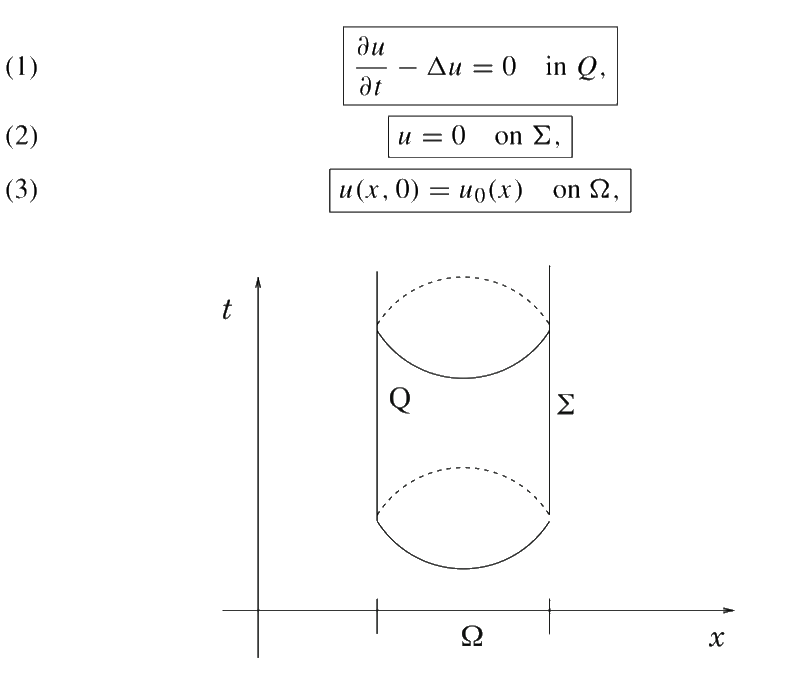
\includegraphics[scale=0.2]{exemple1.png}
\captionof{figure}{Equation de la chaleur sur un ouvert $\Omega$}

\end{frame}



\begin{frame}{Exemple (2)}

On considère de même le cas où la valeur de $u$ est fixée le long de la frontière $\Sigma$. \\~\\


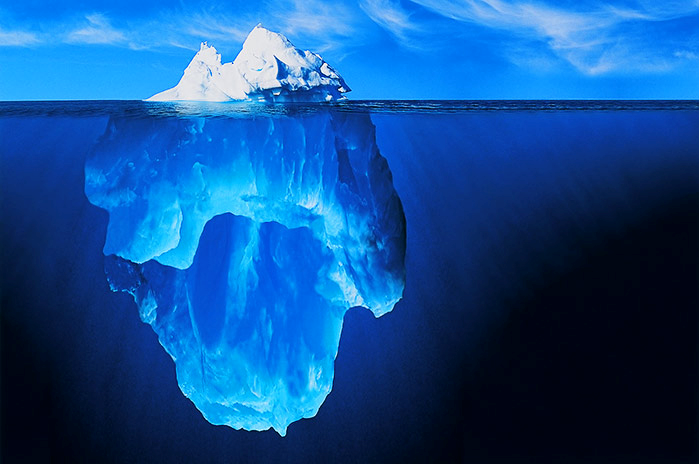
\includegraphics[scale=0.25]{iceberg.png}
\captionof{figure}{Système en contact avec un thermostat} ~ \\~\\

Autre exemple historique : tore métallique dans du sable, pas d'échange avec l'extérieur. Effet régularisant de l'équation de la chaleur.
\end{frame}


\begin{frame}{Cas auto-adjoint}
\textbf{Théorème (variante Hille-Yosida) : \\}
Soit $A$ un opérateur auto-adjoint maximal monotone.\\
 Alors, $\textcolor{red}{\forall  u_0 \in H}, \ \exists ! u \in \mathcal{C}([0,+\infty[,H) \cap \mathcal{C}^1(]0,+\infty[,H)$ tel que : \\ ~ \\
$(*) \begin{cases}\displaystyle \frac{du}{dt} +Au = 0 \text{\ \ \ \ sur } ]0,+\infty[ \\ u(0)=u_0 \end{cases}$ \\ ~ \\ ~ \\
De plus  $\forall t > 0$, $\|u(t)\|\leq \|u_0\| \ $ et $\ \displaystyle \|\frac{du}{dt}\| \leq  \|Au_0\|$
\end{frame}


\begin{frame}{Fin}

\begin{center}
Merci pour votre attention ! \\~\\
Q\&A
\end{center}

\end{frame}


\end{document}